\begin{center}
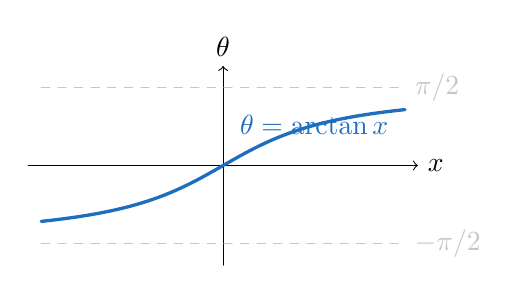
\begin{tikzpicture}[scale=1.1, line cap=round, line join=round]
  \definecolor{trigblue}{RGB}{30,110,190}
  \draw[->] (-2.25,0)--(2.25,0) node[right] {$x$};
  \draw[->] (0,-1.15)--(0,1.15) node[above] {$\theta$};
  \draw[gray!45,dashed] (-2.1,0.9)--(2.1,0.9) node[right] {$\pi/2$};
  \draw[gray!45,dashed] (-2.1,-0.9)--(2.1,-0.9) node[right] {$-\pi/2$};
  \draw[very thick,trigblue,domain=-2.1:2.1,samples=90]
    plot ({\x},{0.9*atan(\x)/90});
  \node[trigblue] at (1.05,0.47) {$\theta=\arctan x$};
\end{tikzpicture}
\end{center}
